\chapter{PHÂN TÍCH VÀ THIẾT KẾ KIẾN TRÚC HỆ THỐNG}
\label{ch:architecture}

\section{Các Quyết định Kiến trúc Cốt lõi}
\label{sec:arch_adrs}

Một hệ thống phần mềm AI hoàn chỉnh không chỉ được đánh giá qua độ phức tạp thuật toán, mà còn thông qua việc cân nhắc thấu đáo các đánh đổi kỹ thuật ở từng tầng thiết kế. Trong quá trình phát triển đồ án, tác giả đã thiết lập 7 bản ghi quyết định kiến trúc (ADR\textsuperscript{2}) làm cơ sở lựa chọn công nghệ và đối sánh trực diện với các lựa chọn thay thế như tổng hợp tại Bảng \ref{tab:framework_comparison}:

\subsection{ADR-001: Lựa chọn Ngôn ngữ Python và Web Framework FastAPI}
\begin{itemize}[leftmargin=1.5cm]
    \item \textbf{Đặt vấn đề:} Máy chủ backend phải đáp ứng đồng thời hai dạng tải trái ngược nhau: (i) giữ kết nối mạng chờ chuỗi 4 tác tử LLM sinh kịch bản tuần tự kéo dài 10--20 giây (tác vụ chờ vào/ra mạng cao), và (ii) duy trì kênh đồng bộ phòng chơi nhóm tối đa 3 thám tử qua WebSocket (\texttt{rooms.py}) song song với các phép tính số học nội tại (giải phương trình Henssge, duyệt đồ thị kiểm chứng, chấm điểm kết án) có độ trễ dưới 5 mili-giây.
    \item \textbf{Các phương án cân nhắc:}
    \begin{enumerate}
        \item \textit{Django (Python):} Đầy đủ tính năng quản trị và kết xuất trang phía máy chủ, nhưng kiến trúc nguyên khối mang theo nhiều thành phần dư thừa đối với dịch vụ định tuyến API thuần JSON và chi phí chuyển ngữ cảnh bất đồng bộ cao.
        \item \textit{Flask (Python):} Gọn nhẹ nhưng mặc định vận hành theo chuẩn giao diện cổng máy chủ đồng bộ (WSGI), làm khóa cứng luồng xử lý của máy chủ trong suốt 10--20 giây chờ phản hồi từ LLM nếu không cấu hình máy chủ phụ trợ phức tạp, đồng thời thiếu cơ chế kiểm chuẩn lược đồ dữ liệu tự động tích hợp sẵn ở tầng định tuyến.
        \item \textit{Node.js (TypeScript):} Xử lý vào/ra bất đồng bộ tốt, nhưng không tương thích trực tiếp với hệ sinh thái tính toán khoa học, phân tích thực nghiệm (\texttt{pandas}, \texttt{matplotlib}) và các thư viện AI bằng Python của phần lõi backend.
        \item \textit{FastAPI (Python 3.13):} Framework hiệu năng cao xây dựng trên chuẩn giao diện máy chủ bất đồng bộ và Pydantic \cite{fastapi2024}.
    \end{enumerate}
    \item \textbf{Quyết định Kiến trúc:} Lựa chọn \textbf{FastAPI trên nền Python 3.13} (phiên bản cài đặt thực tế FastAPI 0.137.1 trên máy chủ Uvicorn 0.49.0).
    \item \textbf{Lý do lựa chọn:} Vòng lặp sự kiện bất đồng bộ nguyên bản (\texttt{async/await}) cho phép máy chủ xử lý nhiều phiên sinh kịch bản và kết nối WebSocket cùng lúc mà không làm nghẽn tiến trình khi chờ LLM; tích hợp trực tiếp Pydantic v2 ngay tại tầng định tuyến HTTP để tự động từ chối gói tin sai cấu trúc; và tự động sinh tài liệu đặc tả OpenAPI tại \texttt{/docs} phục vụ đồng bộ hợp đồng dữ liệu với Unity Client.
\end{itemize}

\subsection{ADR-002: Lựa chọn Thư viện Kiểm chuẩn Dữ liệu Pydantic v2}
\begin{itemize}[leftmargin=1.5cm]
    \item \textbf{Đặt vấn đề:} Đầu ra từ LLM có thể gặp lỗi cú pháp định dạng JSON, thiếu trường bắt buộc, sai định dạng giờ 24 giờ hoặc vượt ngưỡng sinh học hợp lý. Hệ thống cần một tầng kiểm chuẩn lược đồ nghiêm ngặt ngay tại cổng tiếp nhận.
    \item \textbf{Các phương án cân nhắc:}
    \begin{enumerate}
        \item \textit{Thư viện chuẩn \texttt{dataclasses} (Python):} Chỉ định nghĩa cấu trúc lưu trữ thuộc tính, không hỗ trợ tự động ép kiểu hay kiểm tra ràng buộc miền giá trị khi giải mã chuỗi JSON thô từ LLM.
        \item \textit{Marshmallow:} Hỗ trợ kiểm chuẩn lược đồ nhưng thực thi hoàn toàn trên trình thông dịch Python nên tốc độ phân giải chậm hơn đáng kể và buộc lập trình viên phải khai báo tách rời lớp mô hình dữ liệu với lớp lược đồ xác thực.
        \item \textit{Pydantic v2} (phiên bản cài đặt thực tế 2.14.3) \cite{pydantic2024}.
    \end{enumerate}
    \item \textbf{Quyết định Kiến trúc:} Lựa chọn \textbf{Pydantic v2} làm hợp đồng dữ liệu xuyên suốt từ tầng gọi tác tử LLM đến tầng giao tiếp API.
    \item \textbf{Lý do lựa chọn:} Lõi xác thực \texttt{pydantic-core} biên dịch bằng ngôn ngữ Rust mang lại tốc độ phân giải JSON nhanh hơn rõ rệt so với kiểm tra thuần Python; cho phép khai báo ràng buộc miền giá trị trực tiếp trên thuộc tính (như \texttt{Field(ge=30.0, le=200.0)} cho cân nặng và \texttt{Field(ge=0.3, le=2.0)} cho hệ số làm lạnh), kiểm định chuẩn hóa giờ \texttt{HH:MM} qua \texttt{@field\_validator}, cũng như đối sánh biểu thức chính quy (như kiểm tra định dạng giờ \texttt{\textasciicircum(\textbackslash d\{1,2\}):(\textbackslash d\{2\})(?::\textbackslash d\{2\})?\textdollar} hay quy ước mã thực thể \texttt{\textasciicircum SUSP-\textbackslash d\{2\}\textdollar}) để ngắt sớm các dữ liệu hỏng cú pháp trước khi đi vào bộ kiểm định ký hiệu.
\end{itemize}

\subsection{ADR-003: Thiết kế Kiến trúc Dịch vụ Web Kết hợp Client Unity 6 URP 2D Đa nền tảng}
\begin{itemize}[leftmargin=1.5cm]
    \item \textbf{Đặt vấn đề:} Ở giai đoạn thử nghiệm ban đầu, tôi đã xây dựng nguyên mẫu giao diện Web bằng React (\texttt{V0/frontend/}). Tuy nhiên, khi chuyển sang hoàn thiện trải nghiệm bàn làm việc thám tử với ánh sáng động, nhiều lớp thẻ ảnh kéo thả, dây chỉ đỏ co giãn và tính năng tìm phòng chơi mạng cục bộ LAN không cần nhập địa chỉ IP thủ công, nguyên mẫu thuần trình duyệt bộc lộ nhiều giới hạn kỹ thuật.
    \item \textbf{Các phương án cân nhắc:}
    \begin{enumerate}
        \item \textit{Thuần Web React:} Dễ truy cập qua trình duyệt nhưng tốn chi phí đồng bộ thao tác kéo thả kết hợp vẽ dây chỉ đỏ trên cây mô hình tài liệu trình duyệt, và bị cơ chế hộp cát bảo mật của trình duyệt (\textit{browser sandbox}) chặn quyền phát gói tin quảng bá UDP ở tầng mạng cục bộ (cổng \texttt{47777} trong \texttt{lan\_discovery.py} và \texttt{LanDiscoveryClient.cs}).
        \item \textit{Unreal Engine 5:} Tối ưu cho đồ họa 3D quy mô lớn nhưng dung lượng bộ cài nặng nề và dư thừa tài nguyên đối với bài toán giao diện bảng ghim 2D/2.5D.
        \item \textit{Godot Engine:} Nhẹ và mã nguồn mở, nhưng hệ thống xử lý hậu kỳ ánh sáng 2D và quy trình đóng gói đồng thời hai đích WebGL và máy trạm chưa thuận tiện bằng hệ sinh thái Unity trong khung thời gian đồ án.
        \item \textit{Kiến trúc Web API kết hợp Unity 6} (bản hỗ trợ dài hạn 6000.5.8f1) trên đường ống kết xuất phổ quát (URP) 2D \cite{unity2024urp}.
    \end{enumerate}
    \item \textbf{Quyết định Kiến trúc:} Tách hệ thống theo mô hình \textbf{Dịch vụ Web phân tán} (\texttt{FastAPI} RESTful API, giao thức HTTP/JSON, WebSockets, cấu hình CORS mở rộng) kết hợp Client \textbf{Unity 6 URP 2D} hỗ trợ xuất bản đa nền tảng (mục tiêu trình duyệt WebGL và tệp thực thi độc lập).
    \item \textbf{Lý do lựa chọn:} Giải pháp này vừa duy trì trọn vẹn kiến trúc dịch vụ Web và khả năng xuất bản WebGL trên trình duyệt, vừa cho phép dựng giao diện gắn với không gian bàn điều tra (\texttt{BankersLampController.cs} điều khiển độ sáng bóng sợi đốt, \texttt{CorkboardManager.cs} kéo thả ảnh Polaroid kèm dây chỉ đỏ động thời gian thực), khóa tỉ lệ hiển thị chuẩn $1920\times 1080$ (16:9) và mở khóa socket UDP phục vụ tự động tìm phòng chơi LAN tại cổng \texttt{47777}.
\end{itemize}

\subsection{ADR-004: Lựa chọn Đường ống Đa tác tử Tự chủ thay vì Prompt Nguyên khối hay Khung Trừu tượng Nặng}
\begin{itemize}[leftmargin=1.5cm]
    \item \textbf{Đặt vấn đề:} Biên soạn một vụ án trinh thám hoàn chỉnh đòi hỏi đồng thời cốt truyện, thông số pháp y, lời khai từng nghi phạm, chứng cứ bẻ gãy ngoại phạm và chuỗi lập luận giải đố.
    \item \textbf{Các phương án cân nhắc:} (1) Gọi một câu lệnh nguyên khối duy nhất; (2) Sử dụng các khung điều phối đa tác tử cỡ lớn như \texttt{LangChain} hoặc \texttt{AutoGen} vốn chèn nhiều lớp bọc trung gian làm khó kiểm soát chuỗi chỉ dẫn nguyên bản và phát sinh độ trễ phụ trội; (3) Tự cài đặt đường ống gọn nhẹ kế thừa trực tiếp \texttt{AsyncOpenAI}.
    \item \textbf{Quyết định Kiến trúc:} Phân rã quá trình sinh thành \textbf{4 tác tử chuyên biệt chạy tuần tự}: \texttt{OutlineAgent} $\to$ \texttt{CharacterAgent} $\to$ \texttt{ClueAgent} $\to$ \texttt{DeductionAgent}, cài đặt trực tiếp trên lớp nền \texttt{BaseAgent} trong \texttt{agents.py}.
    \item \textbf{Lý do lựa chọn:} Chia nhỏ gánh nặng suy luận cho LLM theo từng lược đồ JSON hẹp giúp tỷ lệ hợp lệ cú pháp đạt 100\% trong thực nghiệm; tách biệt khâu thiết lập chân lý gốc ở \texttt{OutlineAgent} với khâu tạo lời khai và manh mối ở các tác tử sau; đồng thời cho phép gắn cơ chế tự động chuyển mạch dự phòng ở từng tác tử (\texttt{FALLBACK\_CANDIDATES}) khi mô hình chính gặp lỗi hạn mức hoặc gián đoạn mạng.
\end{itemize}

\subsection{ADR-005: Lựa chọn Cơ chế Sửa lỗi Cục bộ}
\begin{itemize}[leftmargin=1.5cm]
    \item \textbf{Quyết định Kiến trúc:} Thay vì hủy toàn bộ hồ sơ và sinh lại từ đầu khi có lỗi logic, bộ điều phối áp dụng cơ chế sửa lỗi cục bộ có định hướng theo trường \texttt{component} (\texttt{outline}, \texttt{character}, \texttt{clue}) của \texttt{ConstraintViolation}.
    \item \textbf{Lý do lựa chọn:} Chỉ tái xử lý thành phần phát sinh lỗi với ngữ cảnh thu gọn hằng số $\mathcal{O}(1)$, hạn chế chi phí token và thời gian khôi phục so với tái sinh toàn bộ đường ống $\mathcal{O}(N)$.
\end{itemize}

\subsection{ADR-006: Điều phối Mô hình qua Cổng Proxy Gateway Cục bộ}
\begin{itemize}[leftmargin=1.5cm]
    \item \textbf{Đặt vấn đề:} Thực nghiệm đối sánh đòi hỏi gọi nhiều dòng mô hình khác nhau (OpenAI GPT, Google Gemini/Gemma, mô hình cục bộ Ollama) qua cùng một giao diện lập trình thống nhất, xử lý giới hạn tốc độ và tách biệt khóa xác thực thay vì duy trì nhiều bộ công cụ phát triển riêng lẻ cho từng nhà cung cấp.
    \item \textbf{Quyết định Kiến trúc:} Kết nối qua cổng Proxy Gateway cục bộ (\texttt{9Router}) tại địa chỉ \texttt{http://localhost:20128/v1}, tương thích chuẩn giao thức OpenAI.
    \item \textbf{Lý do lựa chọn:} Cho phép chuyển đổi mô hình linh hoạt ở thời điểm chạy qua API \texttt{POST /api/settings} hoặc chuyển hướng dự phòng sang máy chủ Ollama nội bộ (\texttt{http://localhost:11434/v1}) mà không cần chỉnh sửa mã nguồn các tác tử, đồng thời hỗ trợ ghi nhận thời gian phản hồi thực tế phục vụ đánh giá thực nghiệm.
\end{itemize}

\subsection{ADR-007: Lựa chọn Cơ sở dữ liệu Quan hệ Nhúng SQLite (Chế độ WAL) và SQLAlchemy 2.0}
\begin{itemize}[leftmargin=1.5cm]
    \item \textbf{Đặt vấn đề:} Hệ thống cần lưu trữ bền vững hồ sơ vụ án, lịch sử kết án của người chơi và nhật ký thực nghiệm benchmark, bảo đảm tính toàn vẹn tham chiếu giữa vụ án và các lượt phá án nhưng không làm phức tạp hóa quá trình đóng gói khi phân phối trò chơi tới người dùng cuối.
    \item \textbf{Các phương án cân nhắc:}
    \begin{enumerate}
        \item \textit{Lưu tệp JSON rời thuần túy:} Dễ gặp rủi ro hỏng tệp khi nhiều luồng ghi đồng thời và không hỗ trợ truy vấn thống kê độ khó theo thời gian thực.
        \item \textit{Hệ quản trị khách--chủ PostgreSQL hoặc MySQL:} Mạnh mẽ cho hệ thống lớn nhiều máy chủ, nhưng đòi hỏi người dùng phải cài đặt dịch vụ cơ sở dữ liệu nền hoặc Docker, không phù hợp với mục tiêu triển khai gọn nhẹ kèm gói trò chơi thực thi độc lập.
        \item \textit{Cơ sở dữ liệu phi quan hệ MongoDB:} Lưu tài liệu JSON tự nhiên nhưng thiếu cơ chế ràng buộc khóa ngoại cưỡng bức và xóa dây chuyền ở tầng lưu trữ giữa hồ sơ vụ án với lịch sử kết án.
        \item \textit{SQLite chế độ WAL kết hợp SQLAlchemy 2.0} (phiên bản cài đặt 2.0.51).
    \end{enumerate}
    \item \textbf{Quyết định Kiến trúc:} Sử dụng \textbf{SQLite} bật cơ chế ghi nhật ký trước (WAL\textsuperscript{23}) làm tầng lưu trữ quan hệ nhúng thông qua thư viện ánh xạ đối tượng -- quan hệ \textbf{SQLAlchemy 2.0}.
    \item \textbf{Lý do lựa chọn:} Chỉ thị \texttt{PRAGMA journal\_mode=WAL} cho phép nhiều luồng đọc đồng thời không bị khóa bởi thao tác ghi trong chế độ phối hợp nhóm 3 người chơi; \texttt{PRAGMA foreign\_keys=ON} bảo đảm tính toàn vẹn tham chiếu \texttt{ON DELETE CASCADE} giữa bảng \texttt{cases} và \texttt{deduction\_logs} đạt chuẩn ACID; đồng thời toàn bộ cơ sở dữ liệu gói gọn trong một tệp đơn lẻ không cần cài đặt máy chủ phụ trợ.
\end{itemize}

\begin{table}[H]
\centering
\caption{Đối sánh Tổng hợp Lựa chọn Công nghệ và Framework Theo Từng Tầng Hệ thống}
\label{tab:framework_comparison}
\begin{tabularx}{\textwidth}{p{2.6cm} p{3.0cm} p{4.0cm} X}
\toprule
\textbf{Tầng Kiến trúc} & \textbf{Công nghệ Chọn} & \textbf{Phương án Đối chứng} & \textbf{Ưu thế Kỹ thuật Quyết định} \\
\midrule
\textbf{Web API \& Điều phối} & FastAPI 0.137.1 (ASGI / Uvicorn) & Flask (WSGI), Django, Node.js & Xử lý bất đồng bộ không khóa luồng khi chờ LLM 10--20s; hỗ trợ WebSocket phòng chơi nhóm và đồng bộ OpenAPI với Python AI. \\
\textbf{Kiểm chuẩn Lược đồ} & Pydantic v2.14.3 (Rust core) & Python \texttt{dataclasses}, Marshmallow & Tốc độ phân giải nhanh nhờ nhân Rust; ép kiểu và bắt lỗi biểu thức chính quy trực tiếp tại biên giới API. \\
\textbf{Điều phối Đa tác tử} & \texttt{BaseAgent} thuần trên \texttt{AsyncOpenAI} & Prompt nguyên khối, LangChain / AutoGen & Kiểm soát trực tiếp prompt và lược đồ JSON hẹp; giảm lớp bọc trung gian; hỗ trợ chuyển mạch dự phòng theo từng tác tử. \\
\textbf{Lưu trữ Dữ liệu} & SQLite (WAL) + SQLAlchemy 2.0.51 & Tệp JSON rời, PostgreSQL, MongoDB & Đạt chuẩn ACID và khóa ngoại \texttt{CASCADE}; đọc/ghi song song không nghẽn nhờ WAL; nhúng gọn không cần cài máy chủ rời. \\
\textbf{Client Đa nền tảng} & Unity 6 URP 2D + REST/WebSocket & Thuần React DOM, Unreal 5, Godot & Vượt giới hạn hộp cát trình duyệt để quét phòng LAN qua UDP cổng \texttt{47777}; kết xuất đèn bàn 2D và dây chỉ đỏ mượt, vẫn hỗ trợ WebGL. \\
\bottomrule
\end{tabularx}
\end{table}

\subsection{Giải trình Phản biện Các Thách thức Kiến trúc}
\begin{enumerate}[leftmargin=1.5cm]
    \item \textbf{Câu hỏi: ``Tại sao không dùng kỹ thuật prompt nâng cao như CoT để ép LLM tuân thủ logic thay vì xây dựng bộ kiểm định tất định?''}
    \begin{itemize}
        \item \textit{Giải trình:} Prompting và CoT chỉ tác động ở tầng gợi ý ngữ cảnh xác suất, không thể bảo đảm bất biến đóng trong không gian nhiều thực thể. Bằng chứng ghi nhận tại Lượt chạy số 5 của mô hình thương mại \texttt{gh/gpt-4o} trong thực nghiệm: dù nhận đầy đủ chỉ dẫn có cấu trúc, tác tử \texttt{ClueAgent} vẫn sinh ra vật chứng \texttt{EV-03} tham chiếu tới nghi phạm \texttt{"UNKNOWN"} không tồn tại. Bộ kiểm định tất định bên ngoài là lớp bảo vệ bắt buộc để phát hiện và chặn loại lỗi này trước khi dữ liệu tới giao diện người chơi.
    \end{itemize}
    
    \item \textbf{Câu hỏi: ``Việc giả định nhiệt độ môi trường $T_{\text{ambient}}$ không đổi trong mô hình Henssge có làm giảm tính thực tế không?''}
    \begin{itemize}
        \item \textit{Giải trình:} Trong giám định y pháp đối với hiện trường phòng kín và khoảng thời gian tử vong dưới 24 giờ, nhiệt độ môi trường ổn định là giả định tiêu chuẩn của biểu đồ Henssge (1988), kèm theo biên độ tin cậy $\pm 1.5$ giờ nhằm hấp thụ sai lệch vi khí hậu nhỏ. Hơn nữa, trong bối cảnh trò chơi suy luận công bằng, việc cung cấp $T_{\text{ambient}}$ xác định giúp người chơi kiểm chứng cửa sổ tử vong dựa trên dữ kiện minh bạch trong hồ sơ.
    \end{itemize}
\end{enumerate}

\section{Kiến trúc Tổng thể Hệ thống}
\label{sec:arch_overview}

Kiến trúc tổng thể của hệ thống (Hình \ref{fig:overall_system_architecture}) được tổ chức theo mô hình ba tầng tách biệt:
\begin{enumerate}[leftmargin=1.5cm]
    \item \textbf{Tầng Giao diện Người dùng (Unity 6 URP 2D):} Triển khai bàn điều tra bảng ghim, hiển thị hồ sơ nạn nhân, thẻ nghi phạm, vật chứng, hỗ trợ kéo thả nối dây chỉ đỏ, các hộp thoại chuyên đề (báo cáo pháp y, phóng đại ảnh, kết án, phòng chơi nhóm qua mạng cục bộ LAN) và ký xác thực yêu cầu mạng qua giao thức HTTP theo kiến trúc REST.
    \item \textbf{Tầng Dịch vụ Cổng vào, Bảo mật và Lưu trữ (FastAPI, Pydantic v2 \& SQLite):} Định tuyến các yêu cầu REST API và kết nối WebSocket đa người chơi, xác thực chữ ký yêu cầu bằng mã xác thực thông điệp dựa trên hàm băm (HMAC\textsuperscript{8}) kèm giải thuật băm an toàn 256-bit (SHA-256\textsuperscript{20}) kèm kiểm tra chống phát lại tại \texttt{ClientIntegrityMiddleware}, kiểm chuẩn kiểu dữ liệu bằng Pydantic v2, quản lý bộ nhớ truy cập ngẫu nhiên (RAM\textsuperscript{18}) và lưu trữ bền vững xuống cơ sở dữ liệu SQLite.
    \item \textbf{Tầng Lõi Lai Neuro-Symbolic:} Điều phối đường ống 4 tác tử sinh nội dung văn học, thực thi tính toán cửa sổ tử vong Henssge, kiểm tra ràng buộc tất định và thực hiện sửa lỗi cục bộ khi có sai phạm.
\end{enumerate}

\begin{figure}[H]
    \centering
    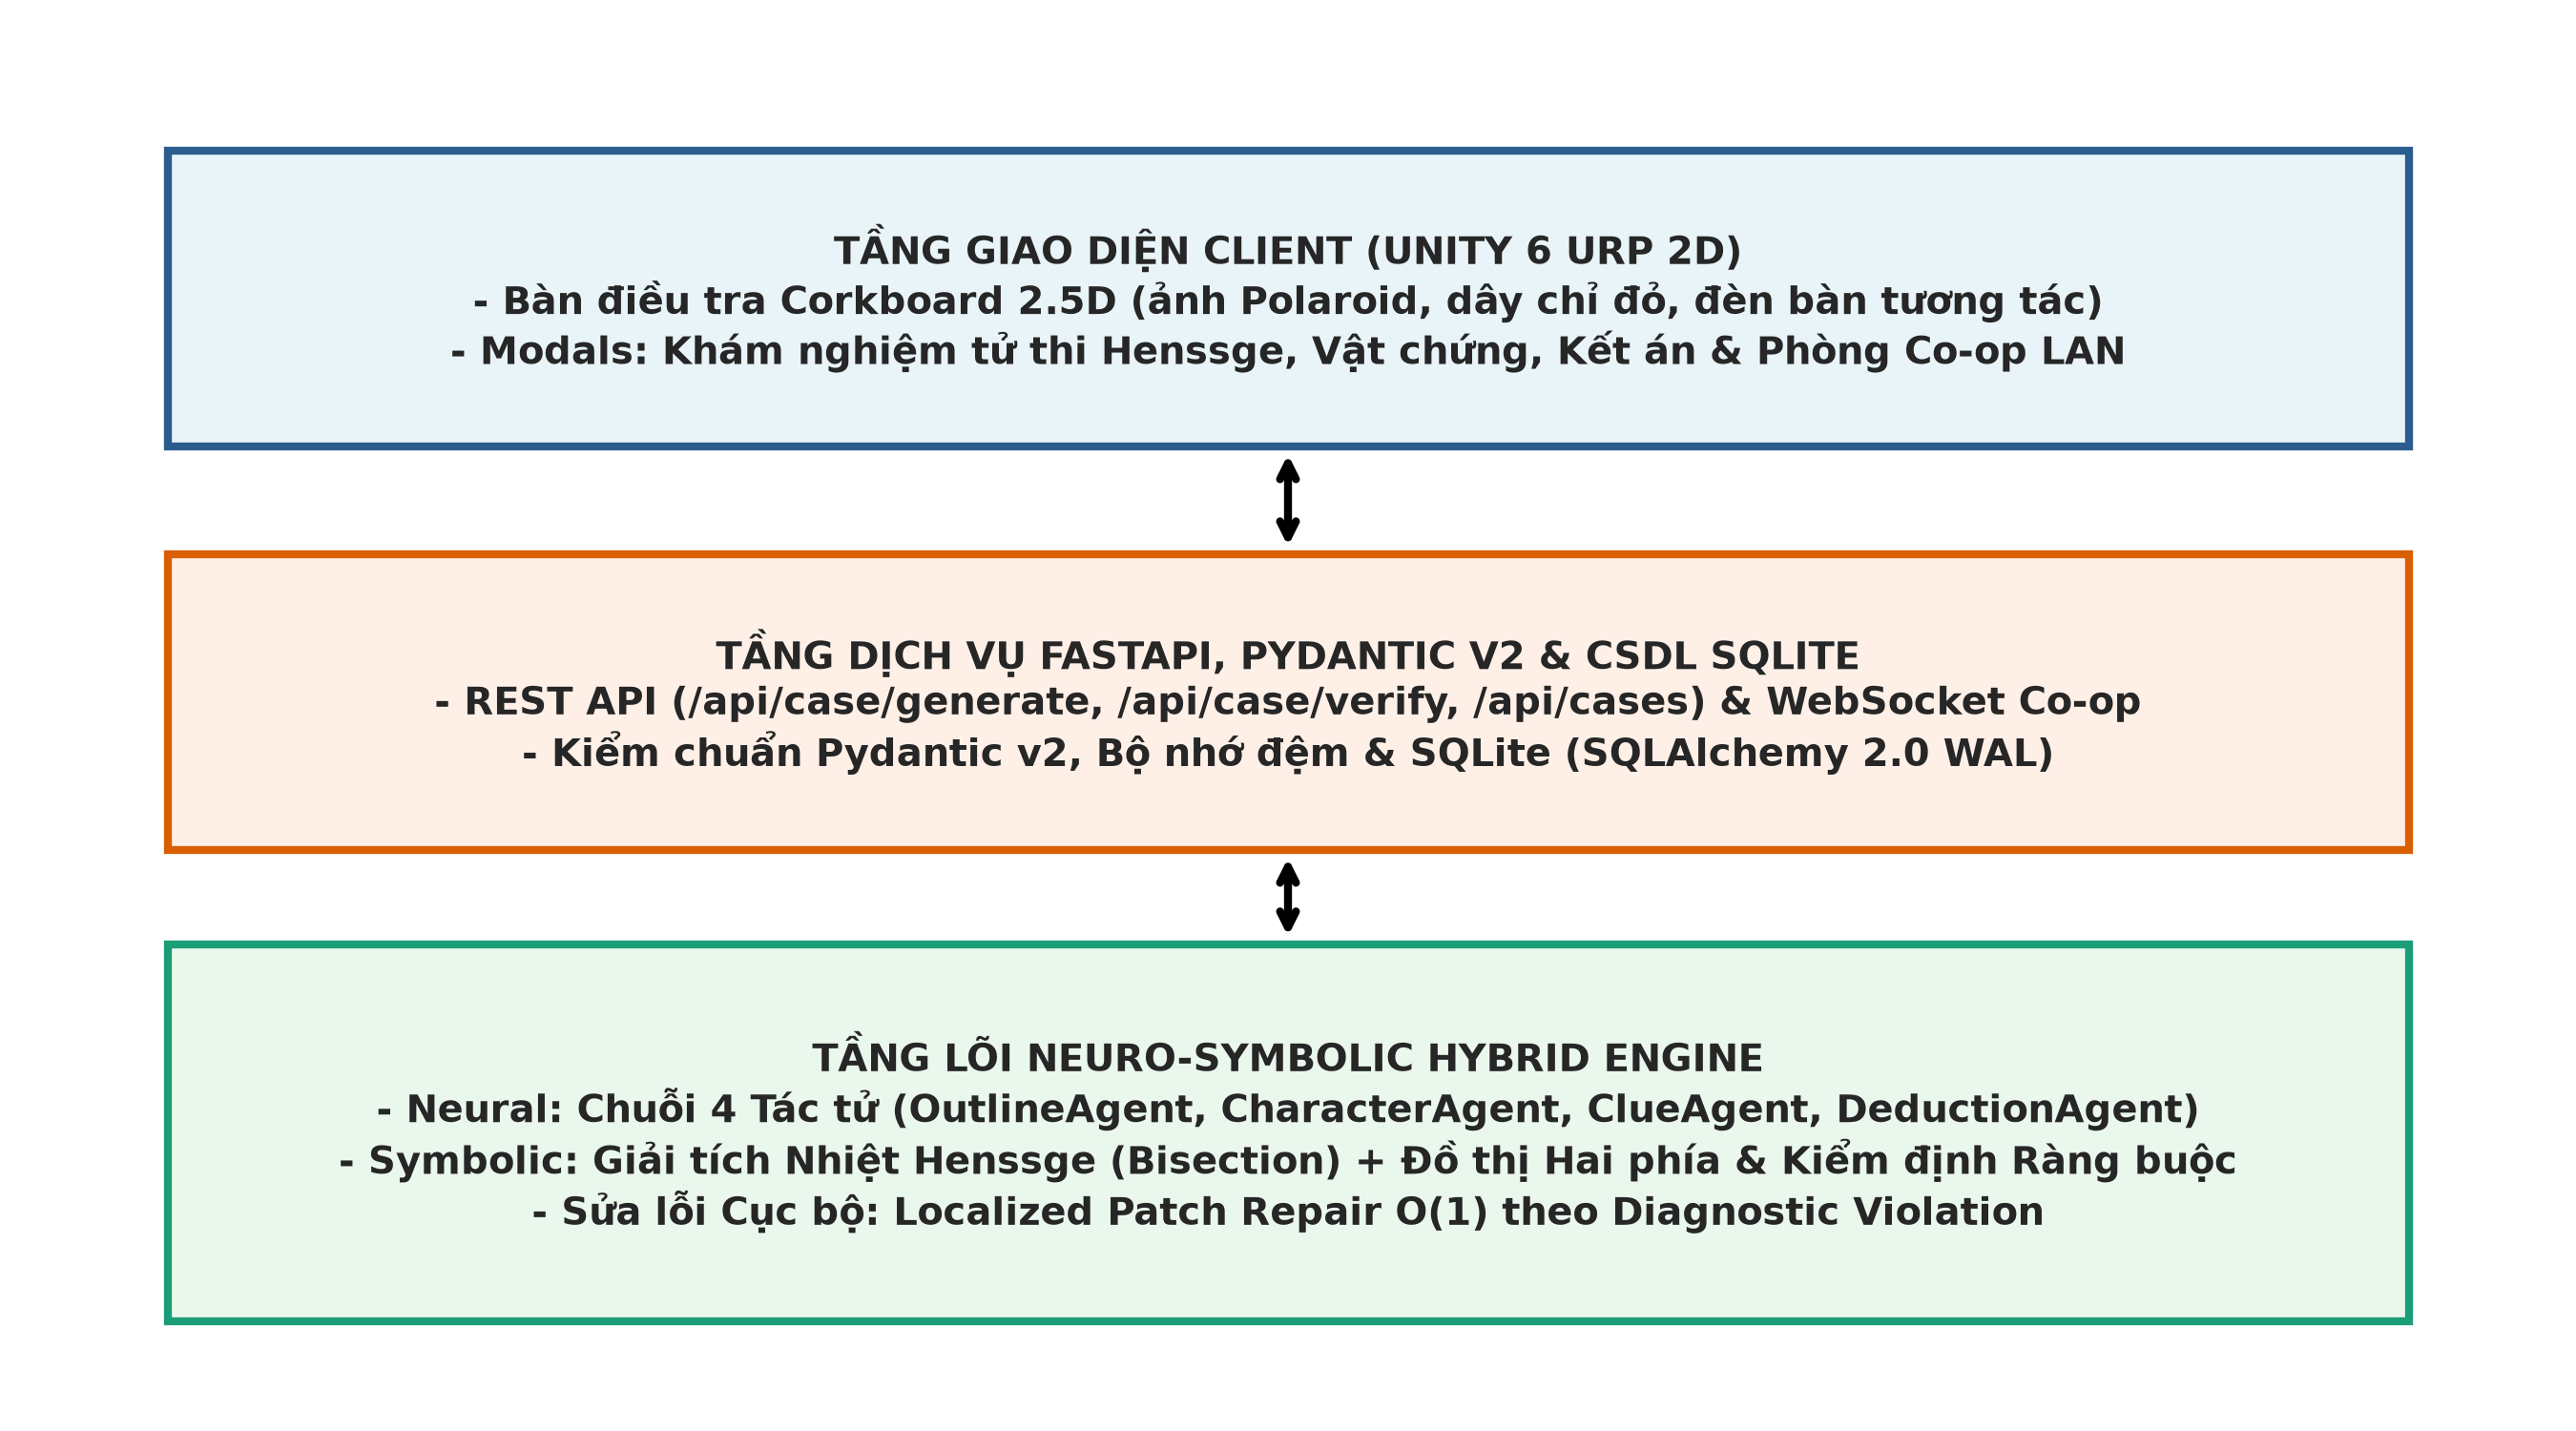
\includegraphics[width=0.95\textwidth]{architecture_overview.png}
    \caption{Sơ đồ Kiến trúc Ba tầng của Hệ thống Trinh thám Neuro-Symbolic}
    \label{fig:overall_system_architecture}
\end{figure}

\section{Thiết kế Luồng Xử lý Dữ liệu và Nguyên lý Phân tách}
\label{sec:arch_data_flow}

Trong mã nguồn hệ thống (\texttt{main.py}, \texttt{llm\_service.py}, \texttt{validator.py}), nguyên lý phân tách trách nhiệm giữa tầng tất định và tầng LLM xác suất được hiện thực hóa qua hai luồng API trọng tâm: luồng tạo sinh hồ sơ vụ án và luồng xác thực phán quyết của người chơi.

\subsection{Luồng Tạo sinh và Kiểm định Vụ án}
Các bước sau mô tả luồng thực thi khi tiếp nhận yêu cầu tới endpoint \texttt{POST /api/case/generate}:
\begin{enumerate}[leftmargin=1.5cm]
    \item \textbf{Khởi tạo ngữ cảnh:} FastAPI tiếp nhận đối tượng \texttt{GenerateCaseRequest} (quốc gia, thời kỳ, địa điểm, thể loại hoặc chủ đề tự do). Nếu bỏ trống chủ đề tự do, hệ thống tự tổng hợp từ danh mục bối cảnh thực tế (\texttt{PRESET\_SETTINGS}) và yêu cầu đặt tên nhân vật thuần bản địa.
    \item \textbf{Sinh khung sườn và khóa vật lý:} \texttt{OutlineAgent} tạo tiêu đề, tóm tắt, hồ sơ nạn nhân (\texttt{Victim}) và chân lý gốc (\texttt{GroundTruth}). Ngay sau bước này, hàm \texttt{apply\_henssge\_tod\_window} trong \texttt{validator.py} tự động tính lại cặp \texttt{estimated\_tod\_start} và \texttt{estimated\_tod\_end} dựa trên phương trình Henssge từ $T_{\text{body}}, T_{\text{ambient}}, M, C$ và giờ phát hiện thi thể. Nhờ đó, động cơ ký hiệu nắm hoàn toàn quyền xác định cửa sổ tử vong chứ không phụ thuộc vào con số ước đoán của LLM.
    \item \textbf{Sinh nghi phạm và vật chứng:} \texttt{CharacterAgent} tạo danh sách nghi phạm (trong đó \texttt{SUSP-01} đóng vai thủ phạm với lời khai che phủ thời điểm gây án); tiếp đó \texttt{ClueAgent} tạo 3--4 vật chứng có chứa manh mối then chốt và manh mối nghi binh.
    \item \textbf{Kiểm định và vá lỗi cục bộ:} \texttt{validate\_case\_diagnostics} rà soát toàn bộ bất biến. Nếu phát hiện lỗi, hệ thống gửi thông báo chẩn đoán tới đúng tác tử chịu trách nhiệm để sửa cục bộ trước khi chuyển sang \texttt{DeductionAgent} sinh chuỗi suy luận nhiều bước (\texttt{ReasoningChain}).
    \item \textbf{Làm giàu tài nguyên và lưu trữ:} \texttt{AssetService} ánh xạ ảnh chân dung nghi phạm và ảnh vật chứng theo từ khóa ngữ nghĩa; \texttt{save\_case\_persistent} lưu hồ sơ xuống SQLite, bộ nhớ đệm RAM và tệp JSON trong thư mục \texttt{cases/}.
\end{enumerate}

\subsection{Luồng Xác thực Kết án Tất định}
Khác với các hệ thống đối thoại để LLM tự đánh giá câu trả lời của người dùng, tại endpoint \texttt{POST /api/case/verify} hệ thống của tôi \textbf{tách biệt hoàn toàn LLM khỏi khâu chấm điểm và tuyên án} nhằm loại bỏ rủi ro phán quyết cảm tính hoặc thay đổi kết quả sai quy tắc. Luồng xử lý gồm 4 bước tuần tự như minh họa ở Hình \ref{fig:sequence_diagram_e2e}:

\begin{figure}[H]
    \centering
    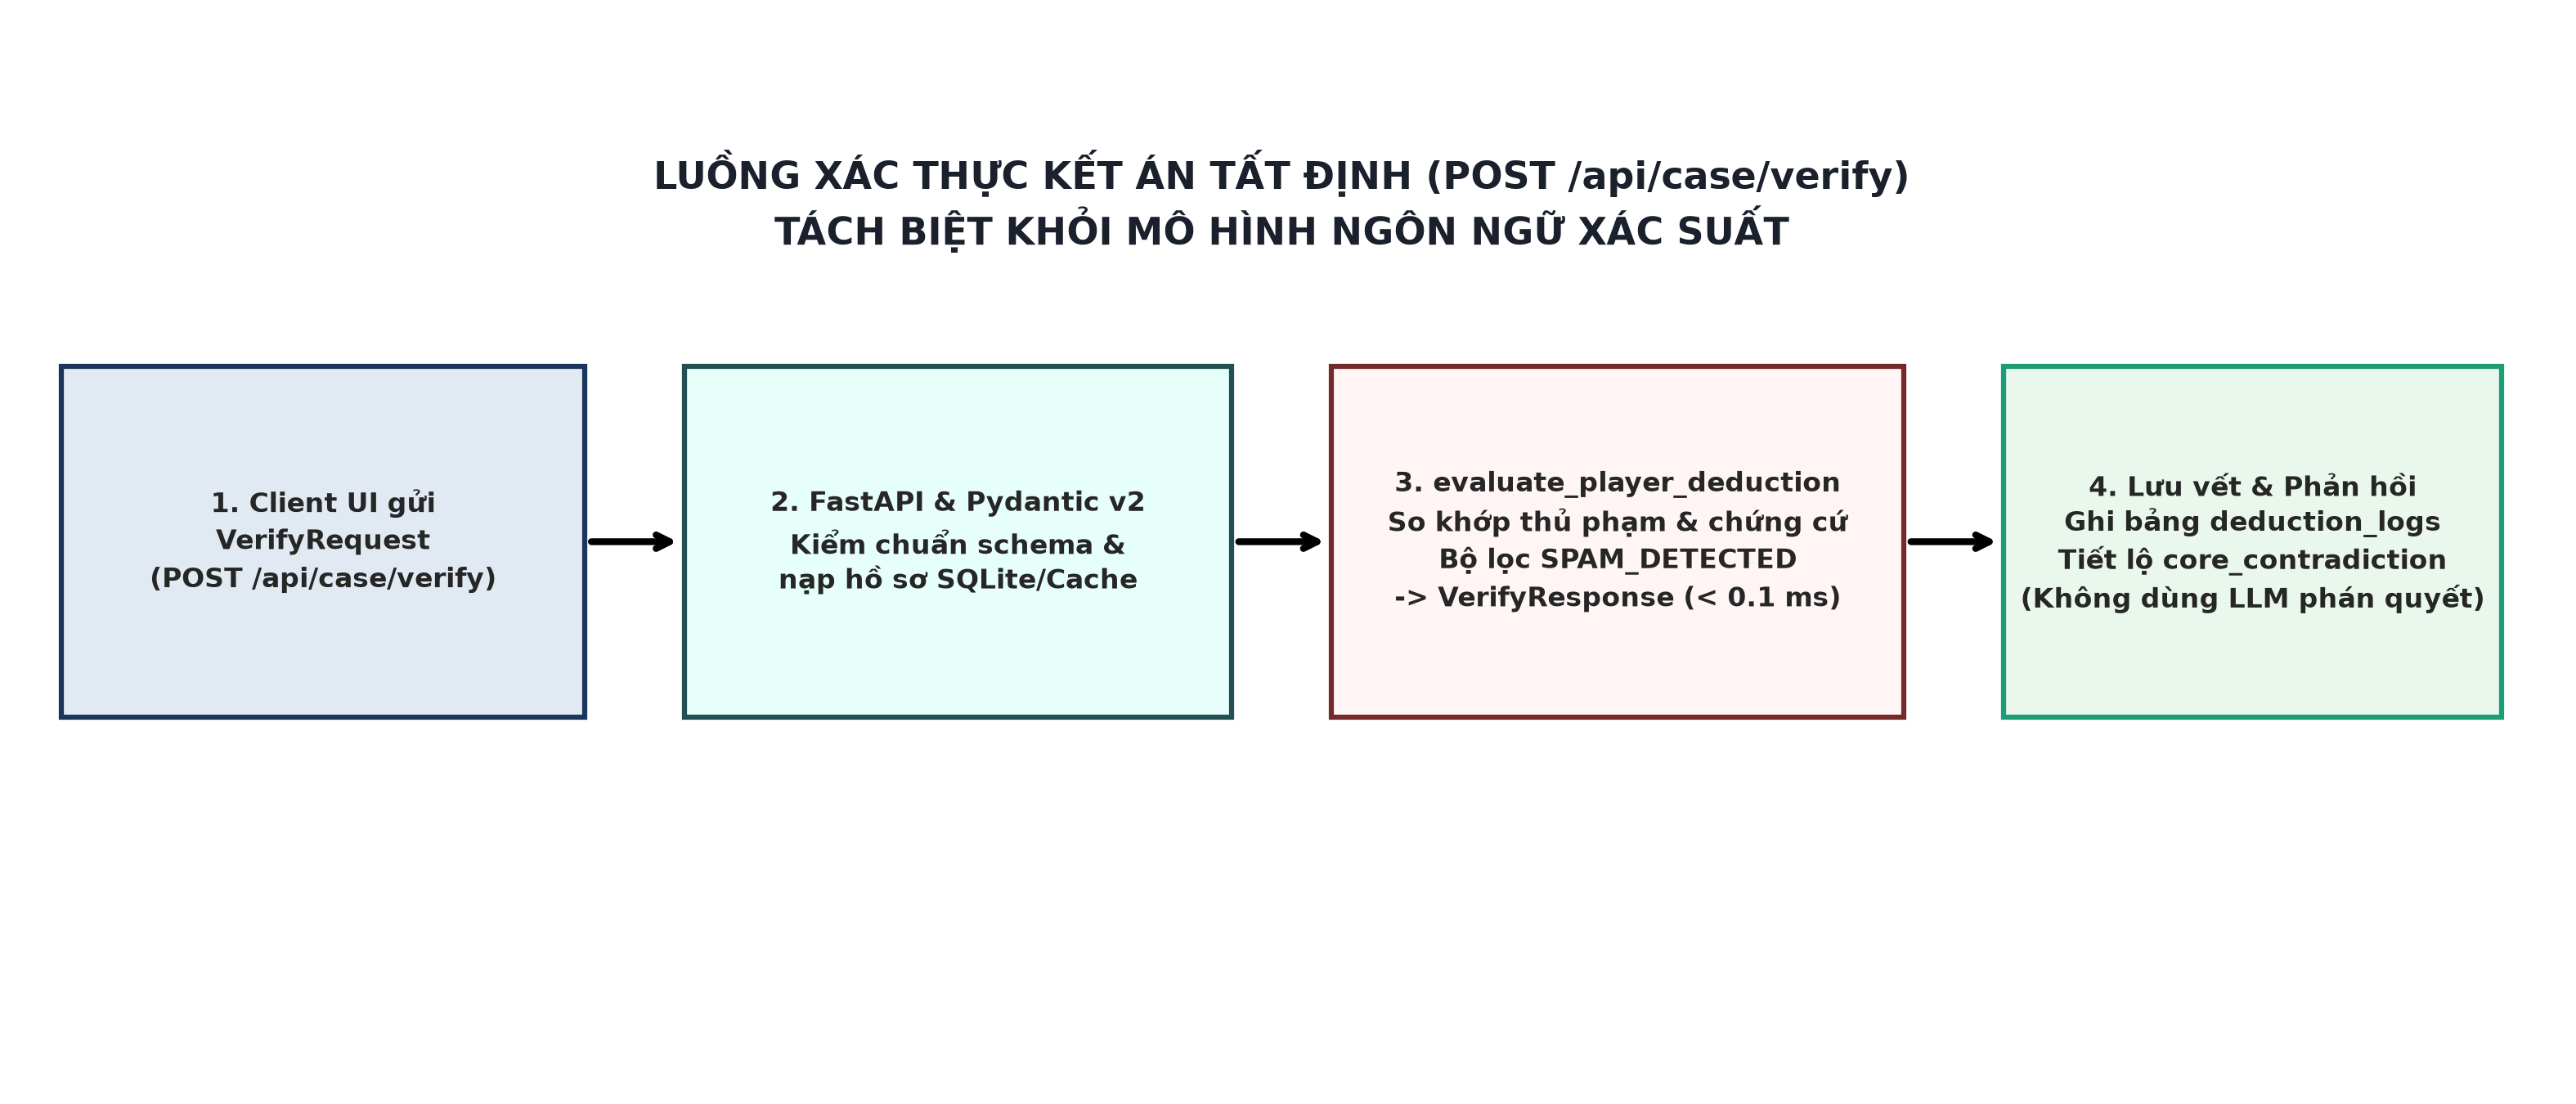
\includegraphics[width=0.95\textwidth]{decoupled_flowchart.png}
    \caption{Luồng Xác thực Kết án Tất định (\texttt{POST /api/case/verify}) Tách biệt Khỏi LLM}
    \label{fig:sequence_diagram_e2e}
\end{figure}

\begin{enumerate}[leftmargin=1.5cm]
    \item \textbf{Tiếp nhận và xác thực tầng biên:} Client UI gửi yêu cầu \texttt{VerifyRequest} (\texttt{case\_id}, \texttt{selected\_suspect\_id}, \texttt{selected\_evidence\_ids}) kèm các tiêu đề chữ ký bảo mật. Middleware đối chiếu chữ ký HMAC-SHA-256 và cửa sổ thời gian 60 giây để ngăn chặn giả mạo hoặc phát lại gói tin, sau đó Pydantic v2 kiểm chuẩn lược đồ dữ liệu và nạp \texttt{CaseDossier} qua \texttt{load\_case\_persistent}.
    \item \textbf{Phán định tất định bằng \texttt{evaluate\_player\_deduction}:} Toàn bộ quá trình chấm điểm thực thi thuần túy trong bộ nhớ RAM với thời gian dưới $0.1\text{ ms}$ dựa trên phép toán tập hợp:
    \begin{equation}
        \text{Verdict}_{\text{logic}} = \left( \text{ID}_{\text{accused}} = \text{ID}_{\text{culprit}} \right) \land \left( |\mathcal{C}_{\text{selected}} \cap \mathcal{C}_{\text{crucial}}| \ge 1 \right) \land \left( |\mathcal{C}_{\text{selected}} \cap \mathcal{C}_{\text{herring}}| = 0 \right)
    \end{equation}
    trong đó hệ thống còn cài đặt bộ lọc chống nộp bừa: nếu tổng vật chứng $\ge 3$ và người chơi chọn toàn bộ vật chứng ($|\mathcal{C}_{\text{selected}}| \ge |V_E|$), kết quả bị gán nhãn \texttt{SPAM\_DETECTED} với 0 điểm.
    \item \textbf{Tính điểm thành phần và phân loại kết quả:} Kết quả được lượng hóa qua \texttt{DeductionScoreBreakdown} (thang điểm tối đa 100: 40 điểm xác định đúng thủ phạm, tối đa 40 điểm cho tỷ lệ tìm đúng chứng cứ then chốt, 20 điểm thưởng độ cô đọng giảm 10 điểm cho mỗi chứng cứ thừa, và phạt 25 điểm cho mỗi manh mối nghi binh), đồng thời phân loại thành 6 trạng thái \texttt{DeductionVerdict}: \texttt{SOLVED\_PERFECT}, \texttt{SOLVED\_FLAWED}, \texttt{WRONG\_SUSPECT}, \texttt{INSUFFICIENT\_EVIDENCE}, \texttt{TRAPPED\_BY\_RED\_HERRING} và \texttt{SPAM\_DETECTED}.
    \item \textbf{Ghi nhật ký và phản hồi Client:} Hàm \texttt{log\_deduction\_to\_db} ghi toàn bộ kết quả lượt chơi vào bảng \texttt{deduction\_logs} trong SQLite và trả về \texttt{VerifyResponse}; trường \texttt{core\_contradiction} chỉ được tiết lộ cho người chơi khi kết án đúng.
\end{enumerate}

\begin{table}[H]
\centering
\caption{So sánh Vai trò và Đặc tính Giữa Tầng Ký hiệu Tất định và Tầng LLM}
\label{tab:decoupled_layer_comparison}
\begin{tabularx}{\textwidth}{l X X}
\toprule
\textbf{Đặc tính Kỹ thuật} & \textbf{Tầng Ký hiệu Tất định} & \textbf{Tầng Tạo sinh LLM} \\
\midrule
\textbf{Bản chất tính toán} & Tất định dựa trên quy tắc đóng & Xác suất tự quy hồi \\
\textbf{Chức năng chính} & Tính $TOD$ Henssge, kiểm định 7 mã lỗi, chấm điểm \texttt{evaluate\_player\_deduction} & Sinh cốt truyện, hồ sơ nạn nhân, lời khai nghi phạm, mô tả vật chứng, chuỗi suy luận \\
\textbf{Khả năng kiểm soát sai số} & Chặn cứng đầu vào/ra sai lược đồ và bất biến logic & Có xác suất ảo giác tham chiếu hoặc sai lệch thời gian \\
\textbf{Thời gian thực thi} & $< 5\text{ ms}$ (kiểm định hồ sơ) và $< 0.1\text{ ms}$ (chấm điểm kết án) & Khoảng $2.5\text{ s} - 7.4\text{ s}$ cho mỗi tác tử tùy mô hình \\
\textbf{Chi phí token} & 0 token & Tiêu thụ token theo từng bước gọi tác tử \\
\bottomrule
\end{tabularx}
\end{table}

\section{Thiết kế Đường ống Đa tác tử}
\label{sec:arch_multi_agent}

Trong \texttt{agents.py} và \texttt{llm\_service.py}, toàn bộ quy trình sinh kịch bản được thực thi thông qua bốn lớp kế thừa từ \texttt{BaseAgent}, vận hành tuần tự như tổng hợp tại Bảng \ref{tab:multi_agent_mapping}. Lớp \texttt{BaseAgent} chuẩn hóa việc gọi API định dạng JSON (\texttt{response\_format=\{"type": "json\_object"\}}, \texttt{temperature=0.7}) và tiền xử lý loại bỏ khối suy nghĩ nội tại (\texttt{<think>...</think>}) hay ký hiệu markdown trước khi giải mã JSON.

\begin{table}[H]
\centering
\caption{Ánh xạ Trách nhiệm và Ràng buộc của Bốn Tác tử trong Hệ thống}
\label{tab:multi_agent_mapping}
\begin{tabularx}{\textwidth}{p{3.6cm} p{5.4cm} X}
\toprule
\textbf{Tên Tác tử} & \textbf{Đầu ra Cấu trúc} & \textbf{Ràng buộc và Hậu xử lý Tất định} \\
\midrule
\textbf{1. \texttt{OutlineAgent}} & Tiêu đề, tóm tắt, \texttt{Victim} (\texttt{ForensicData}), \texttt{GroundTruth} & Chỉ định \texttt{culprit\_id = "SUSP-01"}, thông số nhiệt học thực tế; sau khi sinh, hàm \texttt{apply\_henssge\_tod\_window} tính và ghi đè cửa sổ $TOD$. \\
\textbf{2. \texttt{CharacterAgent}} & Danh sách \texttt{List[Suspect]} (3 nghi phạm) & Đúng 1 nghi phạm có \texttt{is\_culprit=True} khớp \texttt{culprit\_id}; lời khai của thủ phạm bao trùm \texttt{actual\_crime\_time}; nghi phạm vô tội có \texttt{secret\_innocent\_fact}. \\
\textbf{3. \texttt{ClueAgent}} & Danh sách \texttt{List[Evidence]} (3--4 vật chứng) & Ít nhất 1 vật chứng then chốt (\texttt{is\_crucial=True}) bác bỏ lời khai thủ phạm, tối thiểu 1 vật chứng nghi binh (\texttt{is\_red\_herring=True}). \\
\textbf{4. \texttt{DeductionAgent}} & \texttt{ReasoningChain} gồm 2--3 \texttt{DeductionStep} & Các \texttt{clue\_ids} dẫn chiếu phải tồn tại trong danh sách vật chứng hợp lệ; tổng hợp lập luận chứng minh tính giải được. \\
\bottomrule
\end{tabularx}
\end{table}

\section{Hợp đồng Dữ liệu Thực thể với Pydantic v2}
\label{sec:arch_contracts}

Toàn bộ giao tiếp giữa các tác tử LLM, bộ kiểm định, cơ sở dữ liệu và Unity Client đều được chuẩn hóa thông qua các mô hình dữ liệu Pydantic v2 trong \texttt{detective-backend/models.py}. Mã nguồn dưới đây trích xuất trực tiếp các lược đồ thực thể cốt lõi đang vận hành trong hệ thống:

\begin{lstlisting}[language=Python, caption={Trích đoạn Lược đồ Dữ liệu Thực thể trong \texttt{detective-backend/models.py}}]
from pydantic import BaseModel, Field, field_validator
from typing import List, Optional

class ForensicData(BaseModel):
    ambient_temp: float
    body_temp: float
    livor_mortis_state: str
    wound_description: str
    estimated_tod_start: str
    estimated_tod_end: str
    body_weight_kg: float = Field(default=70.0, ge=30.0, le=200.0)
    cooling_factor: float = Field(default=1.0, ge=0.3, le=2.0)
    discovery_time: Optional[str] = None

class Victim(BaseModel):
    name: str
    age: int = Field(..., ge=1, le=120)
    occupation: str
    forensic_data: ForensicData

class Suspect(BaseModel):
    id: str
    name: str
    age: int = Field(..., ge=1, le=120)
    occupation: str
    motive: str
    alibi_start: str
    alibi_end: str
    alibi_statement: str
    secret_innocent_fact: Optional[str] = None
    is_culprit: bool = False
    image_url: Optional[str] = None

class Evidence(BaseModel):
    id: str
    title: str
    location: str
    description: str
    linked_suspect_id: Optional[str] = None
    is_crucial: bool = False
    is_red_herring: bool = False
    image_url: Optional[str] = None

class GroundTruth(BaseModel):
    culprit_id: str
    actual_crime_time: str
    murder_weapon: str
    core_contradiction: str

class CaseDossier(BaseModel):
    case_id: str
    title: str
    summary: str
    victim: Victim
    suspects: List[Suspect] = Field(..., min_length=2, max_length=5)
    evidences: List[Evidence] = Field(..., min_length=2)
    ground_truth: GroundTruth
    reasoning_chain: Optional[ReasoningChain] = None
    metadata: Optional[GenerationMetadata] = None
\end{lstlisting}

Phía Unity Client (\texttt{Assets/Scripts/Models/CaseData.cs}) ánh xạ song song cấu trúc JSON này sang các lớp C\# tuần tự hóa (\texttt{CaseDossier}, \texttt{VictimData}, \texttt{SuspectData}, \texttt{EvidenceData}, \texttt{GroundTruthData}, \texttt{VerifyRequest}, \texttt{VerifyResponse}) để giải mã an toàn qua \texttt{JsonUtility.FromJson}.

\section{Thiết kế Tầng Lưu trữ Dữ liệu Quan hệ}
\label{sec:arch_database}

Nhằm khắc phục rủi ro mất dữ liệu khi chỉ lưu trữ tạm thời trên RAM, tôi triển khai tầng lưu trữ quan hệ sử dụng \textbf{SQLite} kết hợp thư viện ánh xạ đối tượng -- quan hệ (ORM) \textbf{SQLAlchemy 2.0} (phiên bản cài đặt 2.0.51) tại tệp \texttt{detective-backend/database.py}. Khi khởi tạo kết nối, hệ thống tự động kích hoạt các chỉ thị đồng bộ và toàn vẹn trên SQLite:
\begin{itemize}[leftmargin=1.5cm]
    \item \texttt{PRAGMA foreign\_keys=ON}: Bắt buộc kiểm tra khóa ngoại và xóa dây chuyền;
    \item \texttt{PRAGMA journal\_mode=WAL}: Bật chế độ ghi nhật ký trước (WAL) giúp nhiều luồng đọc đồng thời không bị chặn bởi thao tác ghi khi chơi nhóm;
    \item \texttt{PRAGMA busy\_timeout=5000}: Cho phép chờ tối đa 5 giây trước khi báo khóa cơ sở dữ liệu;
    \item \texttt{check\_same\_thread=False}: Tương thích với mô hình xử lý bất đồng bộ của FastAPI.
\end{itemize}

Ba bảng quan hệ cốt lõi được định nghĩa bằng khai báo kiểu tường minh của SQLAlchemy 2.0:
\begin{enumerate}[leftmargin=1.5cm]
    \item \textbf{Bảng \texttt{cases} (Lớp \texttt{CaseRecord}):} Lưu trữ hồ sơ vụ án đã sinh, khóa chính tự tăng \texttt{id}, mã định danh duy nhất \texttt{case\_id} đánh chỉ mục, tiêu đề, tóm tắt, các siêu dữ liệu lọc (\texttt{country}, \texttt{era}, \texttt{mystery\_type}), \texttt{culprit\_id}, \texttt{actual\_crime\_time}, cờ \texttt{is\_valid}, điểm số \texttt{validator\_score}, số lượng nghi phạm/vật chứng, toàn văn cấu trúc \texttt{dossier\_json} và mốc thời gian tạo/cập nhật.
    \item \textbf{Bảng \texttt{deduction\_logs} (Lớp \texttt{DeductionRecord}):} Lưu toàn bộ lịch sử kết án của người chơi với khóa ngoại \texttt{case\_id} tham chiếu tới \texttt{cases.case\_id} (\texttt{ondelete="CASCADE"}). Bảng ghi lại đối tượng bị cáo buộc (\texttt{accused\_id}), danh sách vật chứng đã nộp (\texttt{selected\_evidence\_ids\_json}), \texttt{verdict}, trạng thái đúng/sai (\texttt{is\_correct}), các biến đếm chi tiết (\texttt{found\_crucial\_count}, \texttt{total\_crucial\_count}, \texttt{red\_herrings\_selected\_count}, \texttt{irrelevant\_clues\_count}), điểm số \texttt{score} và phản hồi. Dữ liệu này cung cấp API thống kê độ khó qua \texttt{GET /api/case/\{case\_id\}/stats}.
    \item \textbf{Bảng \texttt{benchmark\_runs} (Lớp \texttt{BenchmarkRunRecord}):} Lưu dữ liệu đo đạc thực nghiệm gồm mã đợt chạy \texttt{run\_id}, tên mô hình \texttt{model\_name}, thứ tự lượt thử \texttt{trial\_index}, các cờ \texttt{schema\_valid}, \texttt{logic\_valid}, \texttt{repair\_applied}, thời gian thực thi \texttt{latency\_seconds} và danh sách vi phạm \texttt{violation\_types\_json}. Khi hàm \texttt{init\_db()} chạy lúc khởi động, hệ thống tự động đồng bộ các tệp JSON cũ từ thư mục \texttt{cases/} và 30 bản ghi từ \texttt{benchmark\_results.json} vào cơ sở dữ liệu SQLite đạt chuẩn tính nguyên tử, nhất quán, cô lập, bền vững (ACID\textsuperscript{1}).
\end{enumerate}

\section{Động cơ Kiểm định Ràng buộc Ký hiệu}
\label{sec:arch_validator}

Mọi đối tượng \texttt{CaseDossier} sau giai đoạn lắp ráp sơ bộ đều được đưa qua hàm \texttt{validate\_case\_diagnostics(case)} trong \texttt{validator.py}. Hàm này rà soát năm nhóm kiểm tra và trả về \texttt{ValidationResult} chứa danh sách 7 loại vi phạm tường minh thuộc \texttt{ViolationType} (Bảng \ref{tab:violation_taxonomy}).

\begin{table}[H]
\centering
\caption{Danh mục 7 Loại Vi phạm Ký hiệu (\texttt{ViolationType}) trong \texttt{models.py}}
\label{tab:violation_taxonomy}
\begin{tabularx}{\textwidth}{l p{2.2cm} X}
\toprule
\textbf{Mã \texttt{ViolationType}} & \textbf{Phân hệ} & \textbf{Điều kiện Kích hoạt và Ý nghĩa Chẩn đoán} \\
\midrule
\texttt{TOD\_PHYSICS} & \texttt{outline} & Giá trị nhiệt độ phi lý (thi thể nguội hơn phòng hoặc quá 48 giờ chưa nguội tới mức đo, thân nhiệt $\ge 37.5^\circ\text{C}$ khi phòng $< 30^\circ\text{C}$), hoặc độ dài cửa sổ $TOD$ ngoài $[15, 720]$ phút. \\
\texttt{CRIME\_TIME\_OUTSIDE\_TOD} & \texttt{outline} & Thời điểm gây án \texttt{actual\_crime\_time} nằm ngoài cửa sổ tử vong $[TOD_{\text{start}}, TOD_{\text{end}}]$ tính theo Henssge. \\
\texttt{ALIBI\_UNBROKEN} & \texttt{clue} / \texttt{outline} & Thủ phạm khai ngoại phạm che phủ giờ gây án nhưng không có vật chứng then chốt phá vỡ ngoại phạm, hoặc trường \texttt{core\_contradiction} rỗng/quá ngắn ($< 10$ ký tự). \\
\texttt{NO\_CRUCIAL\_CLUE} & \texttt{clue} & Vụ án không có bất kỳ vật chứng nào được gắn cờ \texttt{is\_crucial = True}. \\
\texttt{DUPLICATE\_ID} & \texttt{character} / \texttt{clue} & Phát hiện trùng mã định danh nghi phạm (\texttt{SUSP-*}) hoặc mã vật chứng (\texttt{EV-*}). \\
\texttt{MULTIPLE\_CULPRITS} & \texttt{character} / \texttt{outline} & Số lượng nghi phạm mang cờ \texttt{is\_culprit = True} khác 1, hoặc không khớp với \texttt{ground\_truth.culprit\_id}. \\
\texttt{SCHEMA\_ERROR} & \texttt{clue} / \texttt{reasoning} & Tham chiếu thực thể hỏng: \texttt{Evidence.linked\_suspect\_id} hoặc \texttt{DeductionStep.clue\_ids} trỏ tới mã định danh không tồn tại. \\
\bottomrule
\end{tabularx}
\end{table}

\section{Cơ chế Sửa lỗi Cục bộ}
\label{sec:arch_patch_repair}

Khi \texttt{validate\_case\_diagnostics(candidate\_dossier)} trả về \texttt{is\_valid = False}, thay vì hủy bỏ toàn bộ hồ sơ đang xây dựng, \texttt{CaseGeneratorService} trong \texttt{llm\_service.py} duyệt qua từng \texttt{ConstraintViolation} để định tuyến tín hiệu phản hồi tới đúng tác tử chịu trách nhiệm theo mã \texttt{component} (Thuật toán \ref{alg:patch_repair}).

\begin{algorithm}[H]
\caption{Cơ chế Sửa lỗi Cục bộ Định tuyến theo Phân hệ Vi phạm}
\label{alg:patch_repair}
{\small
\begin{algorithmic}[1]
\Require Hồ sơ ứng viên $D = (\text{victim}, \text{suspects}, \text{evidences}, \text{gt})$, Chẩn đoán $Diag$
\Ensure Hồ sơ sau sửa chữa cục bộ $D$ và kết quả tái kiểm định $Diag$
\If{\textbf{not} $Diag.\text{is\_valid}$}
    \ForAll{$v \in Diag.\text{violations}$}
        \State $fb \gets v.\text{message}$
        \If{$v.\text{component} == \texttt{"clue"}$}
            \State $D.\text{evidences} \gets \text{ClueAgent.repair\_clues}(D.\text{evidences}, D.\text{suspects}, D.\text{gt}, fb)$
        \ElsIf{$v.\text{component} == \texttt{"character"}$}
            \State $D.\text{suspects} \gets \text{CharacterAgent.repair\_suspects}(D.\text{suspects}, D.\text{gt}, fb)$
        \ElsIf{$v.\text{component} == \texttt{"outline"}$}
            \State $(D.\text{victim}, D.\text{gt}) \gets \text{OutlineAgent.repair\_tod}(D.\text{victim}, D.\text{gt}, fb)$
            \State $\text{apply\_henssge\_tod\_window}(D.\text{victim}.\text{forensic\_data})$
        \EndIf
    \EndFor
    \State $Diag \gets \text{validate\_case\_diagnostics}(D)$ \Comment{Tái kiểm định sau khi vá}
\EndIf
\State \Return $(D, Diag)$
\end{algorithmic}
}
\end{algorithm}

\subsection{Phân tích Độ phức tạp Không gian Token \texorpdfstring{$\mathcal{O}(1)$}{O(1)}}
Xét chi phí ngữ cảnh khi khắc phục một lỗi logic đơn lẻ giữa hai chiến lược:
\begin{itemize}[leftmargin=1.5cm]
    \item \textbf{Chiến lược tái sinh toàn bộ:} Nếu gọi lại toàn bộ chuỗi 4 tác tử để tạo vụ án mới từ đầu, lượng token tiêu thụ tỷ lệ với quy mô đầy đủ của hồ sơ $N = T_{\text{Outline}} + T_{\text{Character}} + T_{\text{Clue}} + T_{\text{Deduction}}$, tức độ phức tạp $\mathcal{O}(N)$ (ước tính khoảng 2,500--3,500 tokens cho một vụ án 3 nghi phạm, 3--4 vật chứng).
    \item \textbf{Chiến lược sửa lỗi cục bộ:} Khi cô lập vi phạm vào đúng một phân hệ (\texttt{outline}, \texttt{character}, hoặc \texttt{clue}), ngữ cảnh gửi cho hàm vá (\texttt{repair\_clues}, \texttt{repair\_suspects}, hoặc \texttt{repair\_tod}) chỉ bao gồm lát cắt dữ liệu tối thiểu của thực thể lỗi và thông điệp chẩn đoán $N_{\text{patch}}$ (ước tính khoảng 300--500 tokens cho phần sửa vật chứng/ngoại phạm hoặc thông số pháp y), đạt độ phức tạp ngữ cảnh hằng số $\mathcal{O}(1)$ trên mỗi vi phạm đơn lẻ và giảm đáng kể chi phí so với sinh lại toàn bộ hồ sơ.
\end{itemize}

\section{Thiết kế Giao diện Điều tra trên Unity 6 URP 2D}
\label{sec:arch_unity_ui}

Giao diện phía người chơi được phát triển bằng C\# trên \textbf{Unity 6 URP 2D} với trọng tâm là không gian làm việc thám tử trực quan, kết nối với máy chủ FastAPI qua \texttt{DetectiveAPIManager.cs}:

\begin{enumerate}[leftmargin=1.5cm]
    \item \textbf{Bảng ghim điều tra trung tâm (\texttt{CorkboardManager.cs}):} Tự động sinh thẻ nạn nhân (gắn ruy-băng đen), thẻ chân dung các nghi phạm và thẻ vật chứng dưới dạng ảnh Polaroid có thể kéo thả (\texttt{DraggableCard.cs}). Người chơi có thể ghim nối hai thẻ bất kỳ bằng dây chỉ đỏ động (hiển thị đường nối tạm thời và cập nhật vị trí theo thời gian thực khi kéo thẻ).
    \item \textbf{Cơ chế tải tức thời và dự phòng ngoại tuyến (\texttt{GameController.cs}):} Khi khởi động, Client ưu tiên nạp hồ sơ mẫu cục bộ trong thư mục \texttt{StreamingAssets/sample\_case.json} để hiển thị ngay bảng ghim (độ trễ khởi tạo bằng 0), đồng thời cung cấp hộp thoại \texttt{GenerateCaseModal.cs} để người chơi gửi yêu cầu tạo vụ án mới theo quốc gia, thời kỳ và mô hình LLM mong muốn.
    \item \textbf{Hệ thống cửa sổ chuyên đề và đèn bàn tương tác:} Bao gồm cửa sổ báo cáo khám nghiệm tử thi tích hợp dữ liệu nhiệt học Henssge (\texttt{AutopsyReportModal.cs}, Hình \ref{fig:forensic_modal_screenshot}), cửa sổ phóng đại ảnh chứng cứ (\texttt{PhotoLightboxModal.cs}), cửa sổ chi tiết vật chứng (\texttt{EvidenceDetailModal.cs}), cửa sổ nộp cáo trạng (\texttt{AccusationModal.cs}), và đèn bàn cổ điển (\texttt{BankersLampController.cs}) với hoạt ảnh kéo dây chuỗi hạt, nhấp nháy bóng đèn sợi đốt theo các khoảng trễ $35\text{ ms} / 25\text{ ms} / 35\text{ ms}$ và đàn hồi tắt dần theo hàm $\exp(-7t)\cos(14t)$ trong $0.20\text{ s}$.
    \item \textbf{Chế độ phối hợp nhiều người chơi qua LAN:} Sử dụng \texttt{DetectiveNetworkManager.cs}, \texttt{LanLobbyModal.cs}, \texttt{LanDiscoveryClient.cs} và \texttt{VoiceChatController.cs} để đồng bộ vị trí thẻ bài, trò chuyện văn bản và âm thanh thoại PCM 16-bit qua WebSocket \texttt{/ws/rooms/\{room\_id\}} cho tối đa 3 người chơi trong một phòng.
\end{enumerate}

\begin{figure}[H]
    \centering
    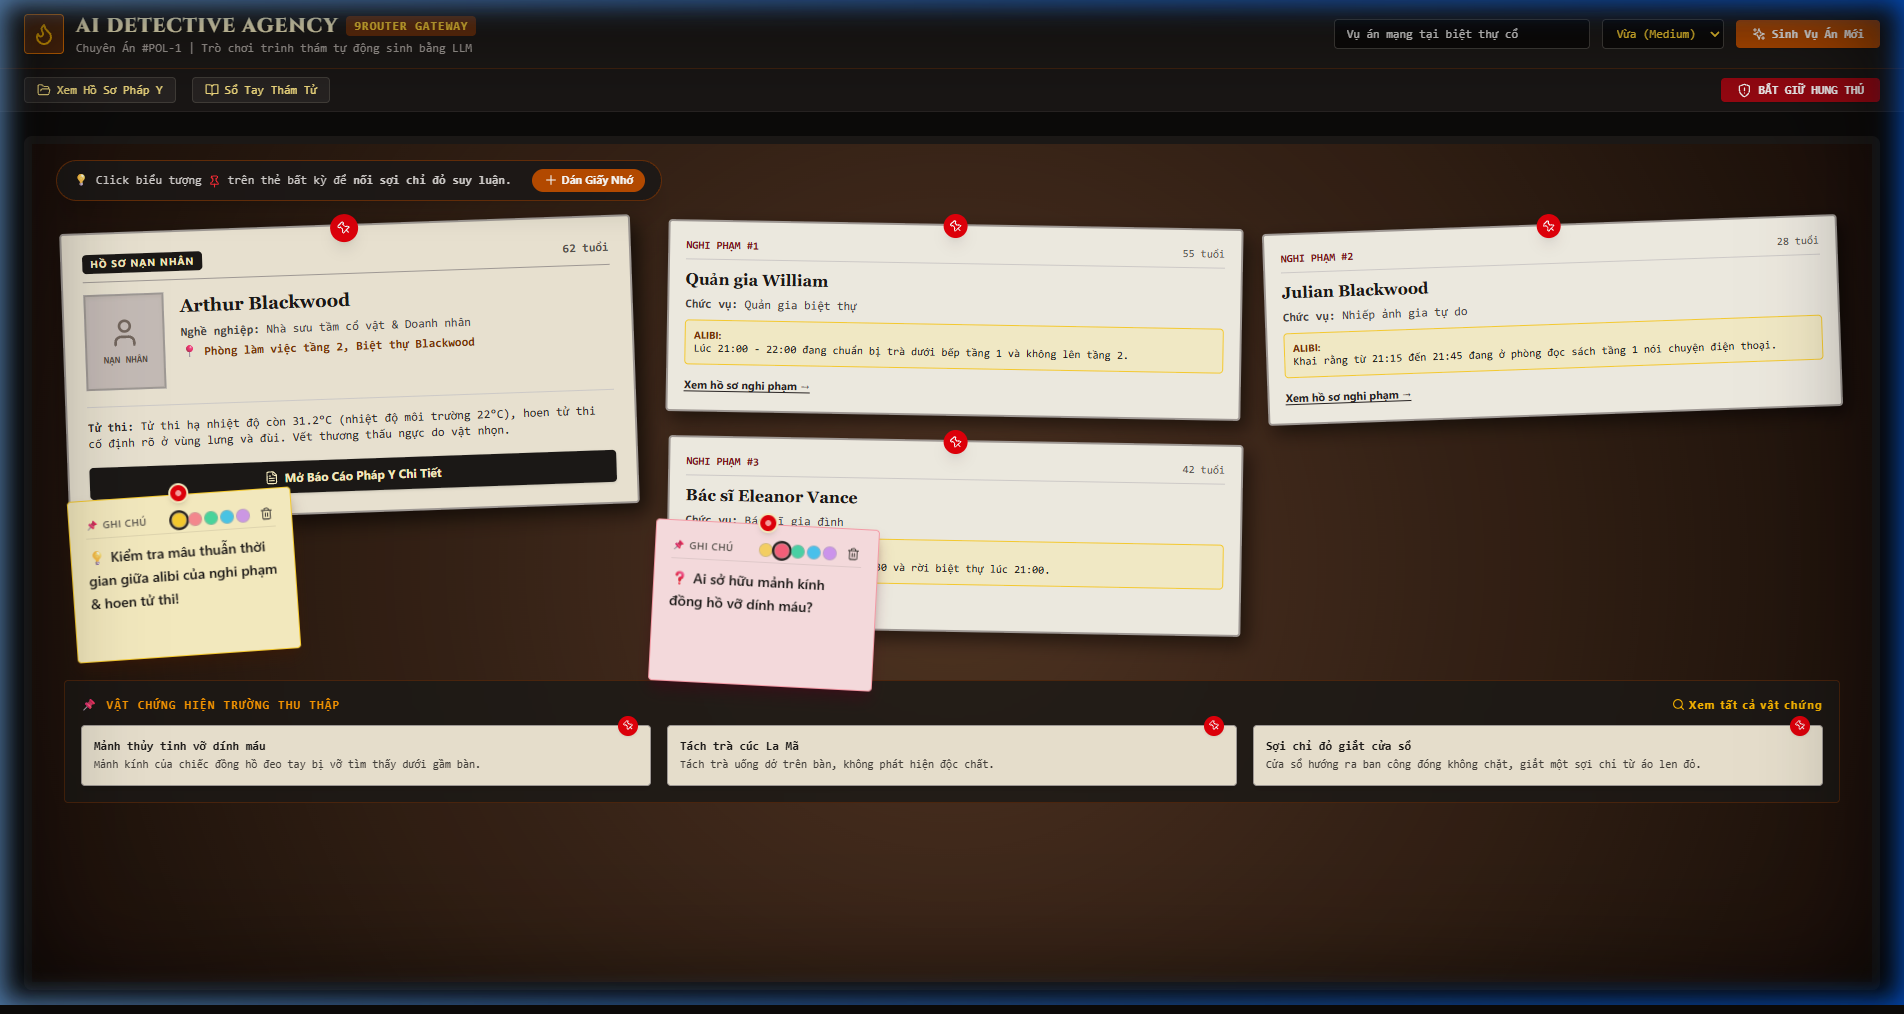
\includegraphics[width=0.95\textwidth]{corkboard_ui.png}
    \caption{Giao diện Bàn Điều tra Corkboard trên Unity 6 URP 2D với Dây chỉ đỏ và Thẻ Hồ sơ}
    \label{fig:corkboard_ui_screenshot}
\end{figure}

\begin{figure}[H]
    \centering
    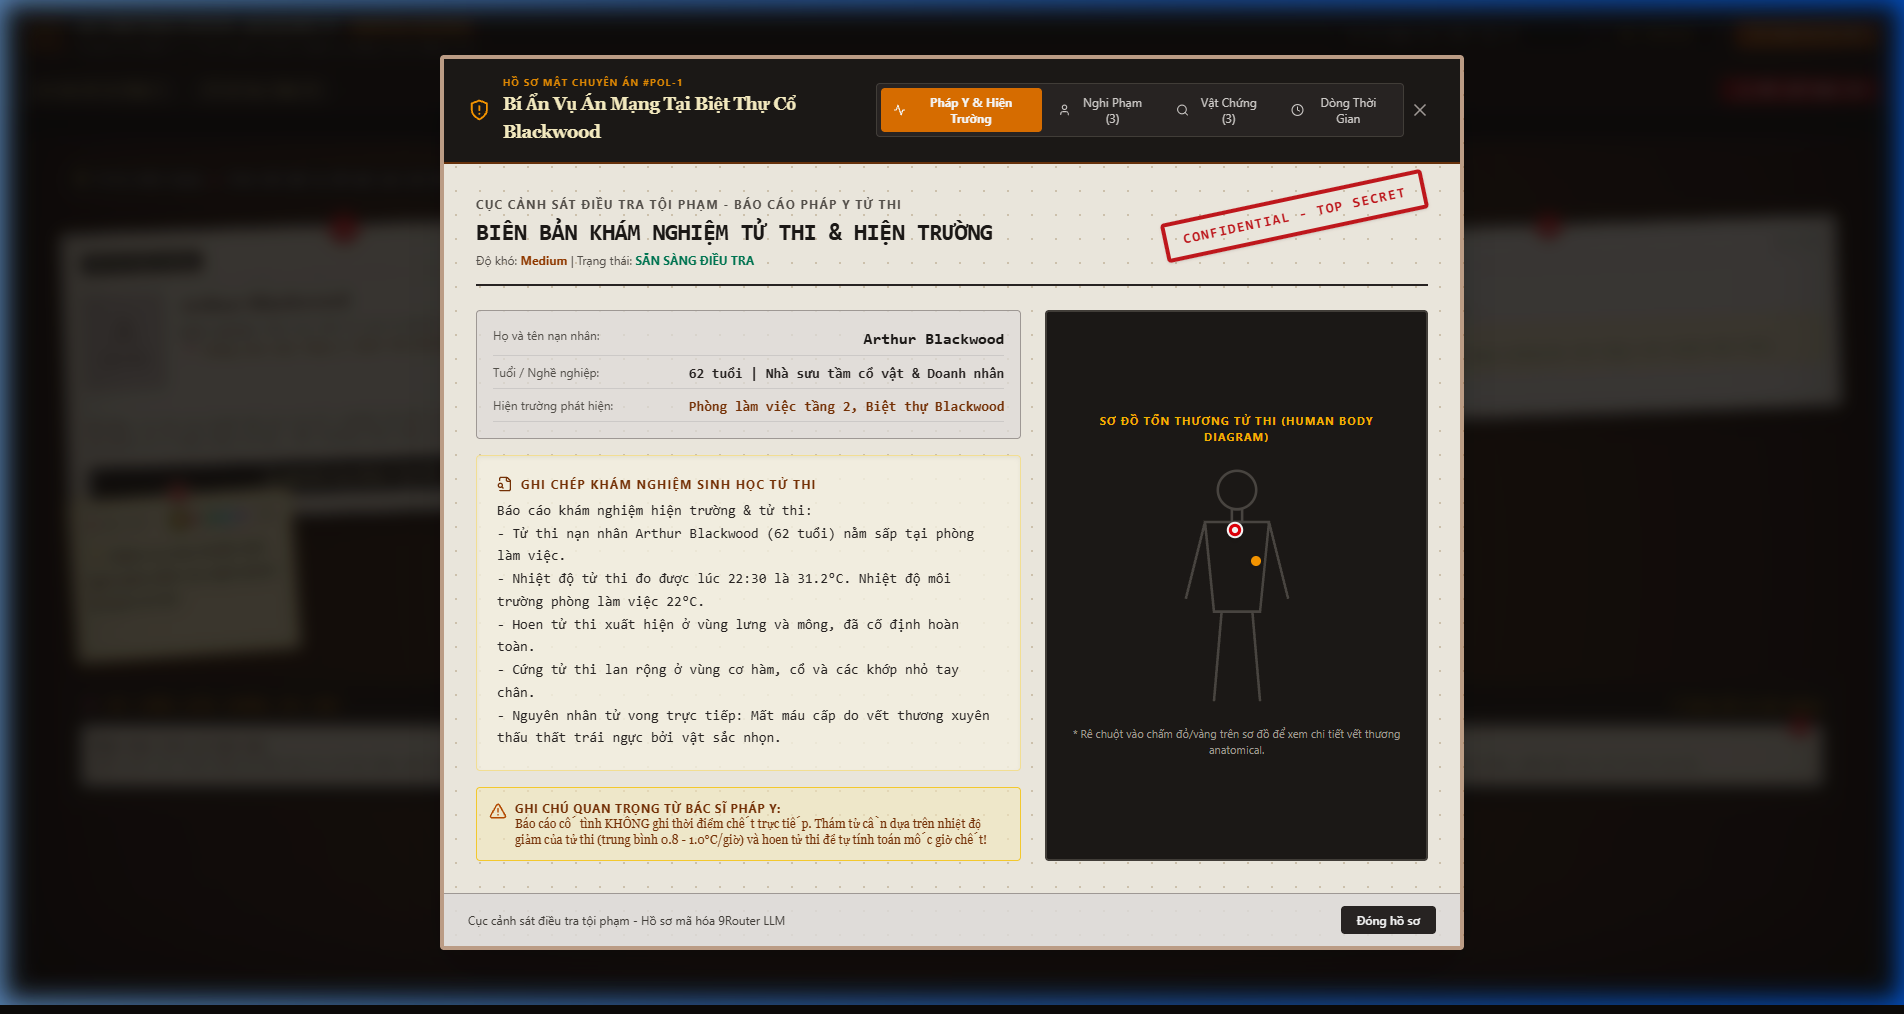
\includegraphics[width=0.85\textwidth]{forensic_modal.png}
    \caption{Giao diện Cửa sổ Báo cáo Khám nghiệm Tử thi Tích hợp Thông số Henssge}
    \label{fig:forensic_modal_screenshot}
\end{figure}
